\onecolumn{}
\begin{figure}
\begin{adjustbox}{minipage={\linewidth},frame}
\vspace{2.5mm}
\centering

\def\picdir{los5d/}
\def\picroc{los5d_ROC.pdf}
\def\piccal{los5d_cal.pdf}
\def\picbar{los5d_SHAP_summary_bar.pdf}
\def\picsum{los5d_SHAP_summary.pdf}
\def\picfpone{los5d_10_SHAP_Pt_5529.png}
\def\picfptwo{los5d_10_SHAP_Pt_1434c2.png}
\def\picfpthr{los5d_10_SHAP_Pt_11022c2.png}

\begin{subfigure}[t]{.45\linewidth}
    \centering
    \captionsetup[subfigure]{}
    \caption[t]{Receiver operator characteristic curve.}\label{fig:roclos5d}
    % 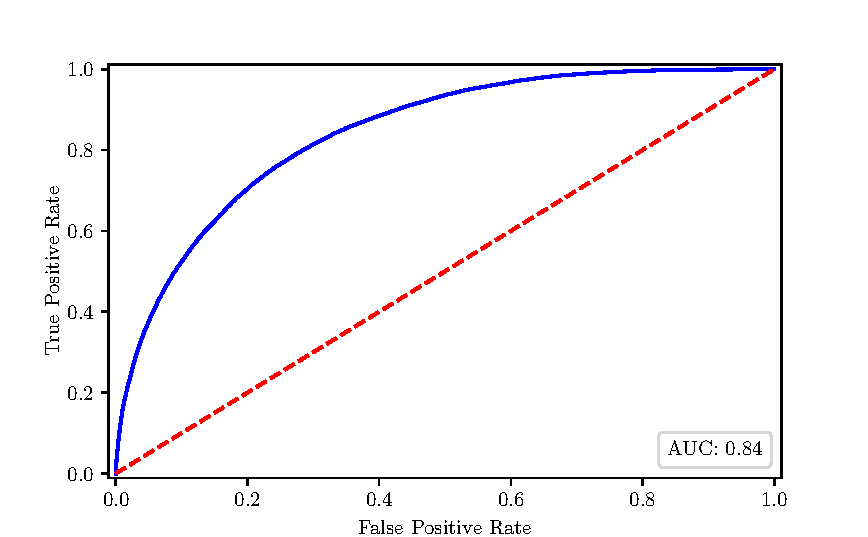
\includegraphics[width=\linewidth,height=.2\textheight,keepaspectratio]{los5d/los5d_ROC.pdf}
    \includegraphics[width=\linewidth,height=.2\textheight,keepaspectratio]{\picdir\picroc}
    % \input{test2.pgf} %% pgf not working for some reason
\end{subfigure}
\begin{subfigure}[t]{.45\linewidth}
    \centering
    \captionsetup[subfigure]{}
    \caption{Calibration curve.}\label{fig:callos5d}
    \includegraphics[width=\linewidth,height=.2\textheight,keepaspectratio]{\picdir\piccal}
    \vspace{2.5mm}
\end{subfigure}

\begin{subfigure}[t]{.45\linewidth}
    \vspace{2.5mm}
    \centering
    \captionsetup[subfigure]{}
    \caption{Bar summary of most impactful features.}\label{fig:shapsumbarlos5d}
    \includegraphics[width=\linewidth,height=.40\textheight,keepaspectratio]{\picdir\picbar}
    % \vspace{2.5mm}
\end{subfigure}
\begin{subfigure}[t]{.45\linewidth}
    \vspace{2.5mm}
    \centering
    \captionsetup[subfigure]{}
    \caption{Summary of most impactful features.}\label{fig:shapsumlos5d}
    \vspace{-2.3mm}
    \includegraphics[width=\linewidth,height=.38\textheight,keepaspectratio]{\picdir\picsum}
    \vspace{2.0mm}
\end{subfigure}
\textsf{Individualized predictions with interpretation.}
\vspace{-2.5mm}
\begin{subfigure}[t]{0.1\textwidth}
    \caption{}\label{fig:shapforcelos5d1}
    \end{subfigure}%
    \begin{minipage}[c]{0.9\textwidth}
    \includegraphics[width=\linewidth,keepaspectratio]{\picdir\picfpone}
    \vspace{-2.5mm}
\end{minipage}
\begin{subfigure}[t]{0.1\textwidth}
    \caption{}\label{fig:shapforcelos5d2}
    \end{subfigure}%
    \begin{minipage}[c]{0.9\textwidth}
    \includegraphics[width=\linewidth,keepaspectratio]{\picdir\picfptwo}
    \vspace{-3.5mm}
\end{minipage}
\vspace{-4.5mm}
\begin{subfigure}[t]{0.1\textwidth}
    \caption{}\label{fig:shapforcelos5d3}
    \end{subfigure}%
    \begin{minipage}[c]{0.9\textwidth}
    \includegraphics[width=\linewidth,keepaspectratio]{\picdir\picfpthr}
    \vspace{-2.5mm}
\end{minipage}
\vspace{-2.5mm}

\caption{\textbf{Length of Stay Over 5 Days.} \\\\
Model performance curves are shown for binary classification (Panel~\ref{fig:roclos5d}) and probability calibration (Panel~\ref{fig:callos5d}).\\\\
Panels~\ref{fig:shapsumbarlos5d} and~\ref{fig:shapsumlos5d} shows the most impactful features on prediction, 
along with the impact of high or low values for numeric features.%
For~\ref{fig:shapsumlos5d}, the line is made of individual dots representing each admission,
and the thickness of the line is determined by the number of examples at a given value (for example, many of our patients are elderly).
A negative SHAP value explains a reduced probability, while a positive one increases it.
For example, advanced age increases the probability of extended length of stay (SHAP value between zero and one), 
while young age tends toward a SHAP value between roughly -1 and zero, corresponding to reduced probability.
For non-numeric features, such as primary diagnosis, the gray points represent specific possible values, with certain diagnoses greatly
increasing or reducing the model's output, while the majority of diagnoses have relatively mild impact on prediction.\\\\
Panels~\ref{fig:shapforcelos5d1}--\ref{fig:shapforcelos5d3} show the composition of invididualized predictions for three patients.
The 75-year-old patient in~\ref{fig:shapforcelos5d1} was admitted to the inpatient service directly from an MD's office with leakage of a heart valve graft.
The patient received 32 medications in the first 24 hours, and has Medicare Part A insurance coverage.
The model predicted the patient's probability of staying longer than five days was 0.80, 
nearly four times the baseline prediction of \textasciitilde0.2.
The majority of the model's prediction was based on the diagnosis, followed by the number of initial medications, and then the other variables as shown.
The patient in~\ref{fig:shapforcelos5d3}, on the other hand, had a predicted probability of length of stay of 0.06, 
or roughly one fourth of the baseline, despite being admitted to the ICU within 24 hours of admission.
The major contributor to this low probability was the diagnosis of antidepressant poisoning, followed by insurance provider,
and, finally, by a lack of BMI recorded in the chart for this encounter.
}\label{fig:los5d}
\end{adjustbox}
\end{figure}